\documentclass{article}
\usepackage[utf8]{inputenc}
\usepackage{amsmath,amsfonts,amssymb,amsthm,mathtools}
\usepackage{parskip}
\usepackage{color}
\usepackage{booktabs}

\newtheorem{exercise}{Exercise}
\newtheorem{answer}{Answer}

\newcommand{\dd}[2][]{\frac{\partial #1}{\partial #2}}
\newcommand{\yh}{\hat{y}}

\newcommand{\bracket}[3]{\left#1 #3 \right#2}
\newcommand{\sqb}{\bracket{[}{]}}
\renewcommand{\b}{\bracket{(}{)}}
\newcommand{\abs}{\bracket{\lvert}{\rvert}}

\newcommand{\x}{\mathbf{x}}
\newcommand{\y}{\mathbf{y}}
\newcommand{\X}{\mathbf{X}}
\newcommand{\I}{\mathbf{I}}

\newcommand{\w}{\mathbf{w}}
\newcommand{\wo}{\w^*}

\renewcommand{\L}{\mathcal{L}}
\newcommand{\E}{\mathbb{E}\sqb}

\title{EMAT31530, Part 2: Linear regression}
\author{Laurence Aitchison}
\date{}

\begin{document}

\maketitle

\section{Regression as curve fitting}
Ultimately, regression is just curve-fitting.
And the simplest form of regression is fitting a straight line to a dataset involving inputs, $x_i$ and targets, $y_i$.
\begin{center}
  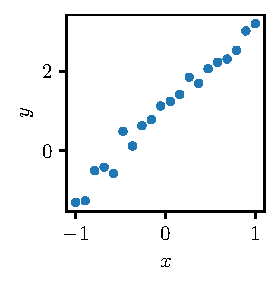
\includegraphics{scatter.pdf}
\end{center}
You can draw a line by hand, or guess a good function in simple cases such as this.
For instance, looking at the plot, we can see that the intercept (where the line crosses $x=0$) is around 1 and the slope is around 2 (it goes up roughly $2$ on the y-axis if we move right $1$ on the x-axis).
Thus, we could guess:
\begin{align}
  \hat{y}(x) = 2 x + 1
\end{align}
where $\hat{y}(x_i)$ is our prediction of the value of $y_i$.
\begin{center}
  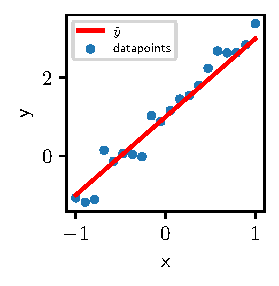
\includegraphics{guess.pdf}
\end{center}
But there are many situations where this simple approach isn't going to work:
\begin{itemize}
  \item Too many datapoints to visualise easily.
  \item Too complicated function to guess.
  \item The input, $x_i$ isn't just one number, but a vector of numbers, $\x_i$ representing multiple ``features'' (for instance, if we're trying to predict sales of a product, our prediction might depend on size, shape, color, weight of a product).
\end{itemize}
In these more complicated contexts, we can't just draw something by eye.
We're going to need to fit the curves using maths!
And it turns out that this curve-fitting is the starting point for AI.

\section{Quantifying good and bad predictions using distances/losses}

To get a mathematical procedure for fitting good predictions, we need to know what makes a good prediction and what makes a bad prediction.
Intuitively, a good prediction is close to the $y_i$'s in the data, and a bad prediction is far from the $y_i$'s in the data.
\begin{center}
  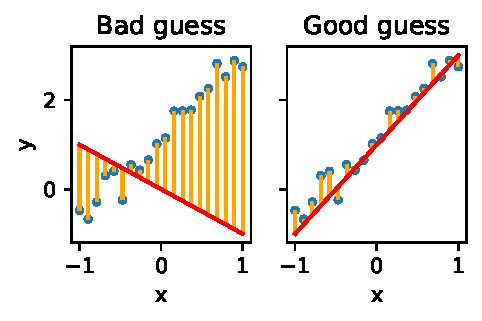
\includegraphics{good_bad.pdf}
\end{center}
But to choose better predictors, we need to formally nail down this notion of distance between the prediction and the data.
Specifically, the goal is to measure the distance between the prediction, $\yh(x_i)$, and the data, $y_i$.
There are a huge number of sensible things we could choose, corresponding to different mathematical formalisations of ``distance''.
Any given notion of distance will give rise to a ``loss'', $\L$. 
Generally speaking, the loss is a sum of distances for each datapoint, because we want the prediction for every datapoint to be close to the data.
Perhaps the most obvious is to use the sum of distances between $y_i$ and $\yh_i$,
\begin{align}
  \L &= \sum_i \abs{\yh(x_i) - y_i},
\end{align}
where,
\begin{center}
  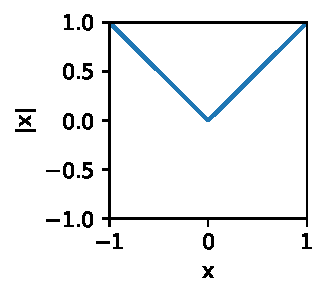
\includegraphics{abs.pdf}
\end{center}
This has lots of nice properties, and is a good option in many cases.
However, the ``kink'' at $x=0$ can cause numerical problems, and can make analytic maths harder.
To make the maths easier, the standard approach is to use the sum of \textit{squared} distances,
\begin{align}
  \L &= \sum_i \b{\yh(x_i) - y_i}^2,
\end{align}
To check that this loss does something sensible, we computed it for the Good Guess/Bad Guess Figure above.  The obviously badly-fitting line (left) has a loss of 34.1 and the obviously better-fitting line (right) has a loss of 4.8.
So the better-fitting line indeed has a lower loss.

\section{Different choices of functions}
We now have a ``loss'' the quantifies how good any given prediction-function, $\yh(x_i)$, is.
In the previous section, we used the loss to show that one particular choice of prediction-function was better than another choice of prediction-function.
So we might want to try loads of different choices of prediction-function, and find the one with the lowest loss.
But that doesn't scale:
\begin{itemize}
  \item Where are these possible prediction-functions going to come from?
  \item What if we have \textit{loads} of possible prediction-functions?
\end{itemize}
To solve these problems, we're going to write our family of possible prediction functions using parameters (NNs will turn out to be the same idea, but where we have \textit{loads} more parameters: usually somewhere between a thousand and a trillion).
For instance we could consider three predictors: the constant predictor, the ``slope'' predictor, and the straight-line predictor,
\begin{align}
  \yh_\text{const}(x_i) &= w_1 & 
  \yh_\text{slope}(x_i) &= w_2 x_i &
  \yh_\text{straight}(x_i) &= w_1 + w_2 x_i.
\end{align}
We can choose different values for the parameters, $w_1$ and $w_2$.
Possible functions in that family are,
\begin{center}
  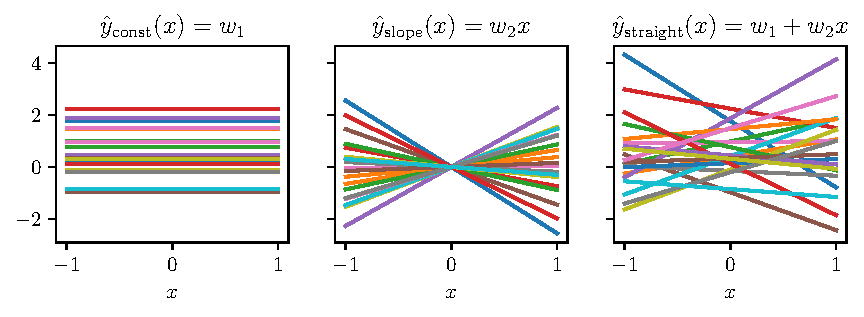
\includegraphics[width=\textwidth]{families.pdf}
\end{center}
There are infinitely many functions in these families, because there are infinitely many possible choices of $w_1$ and $w_2$.
That means we can't try all possible values of $w_1$ and $w_2$.
What can we do instead?
It turns out we can find the lowest-loss function analytically, using calculus.
Remember that the minimum of a function is often where the function has slope $0$.
\begin{center}
  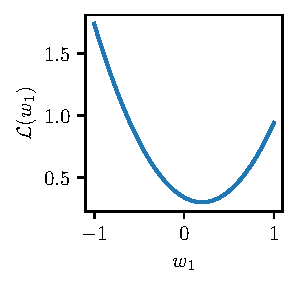
\includegraphics{x2.pdf}
\end{center}

\subsection{Finding the best constant predictor}
The constant predictor always predicts that $y$ is $w_1$,
\begin{align}
  \yh_\text{const}(x_i) &= w_1 & 
\end{align}
That means the loss (sum of squared distances between the prediction and actual value) becomes,
\begin{align}
  \L_\text{const}(w_1) &= \sum_i \b{\yh_\text{const}(x_i) - y_i}^2 =  \sum_i \b{w_1 - y_i}^2
\end{align} 
Our goal is to to find the prediction-function with the lowest loss.
We can do this graphically,
\begin{center}
  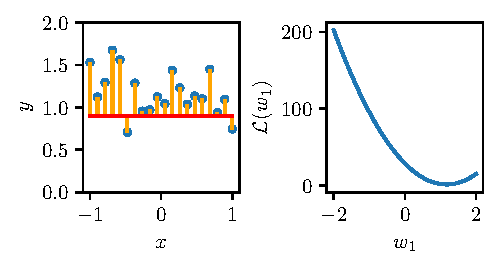
\includegraphics{const_obj.pdf}
\end{center}
and we can see that the optimal value of $w_1$ is about $1.1$, which is about in the middle of the data.


But can we do a better job?
Look at the smooth curve of loss against $w_1$: the minimum of the curve is the location where the gradient is zero.
So, we can find that minimum by treating $\L_\text{const}(w_1)$, as a function of the parameters. 
We find the gradient of $\L_\text{const}(w_1)$, then solve for the value of $w_1$ at which the gradient is zero.
We start by differentating the loss,
\begin{align}
  \label{eq:const:grad_0}
  \dd[\L_\text{const}(w_1)]{w_1} &= \dd{w_1} \sqb{\sum_{i=1}^N \b{y_i - w_1}^2}.\\
  \intertext{(Note I'm playing fast-and-loose with $d$ and $\partial$.  This is done all the time by deep learners, so it is important to be able to work with it.  I'm going to be more careful when we come to talking about backprop in general, where this distinction matters a bit more).  Swap the gradient and the sum,}
  \dd[\L_\text{const}(w_1)]{w_1}  &= \sum_{i=1}^N \dd{w_1} \b{y_i - w_1}^2. %\b{y_i^2  - 2 w_1 y_i + w_1^2}\\
  \intertext{Now, we take $u_i=y_i - w_1$,}
  \dd[\L_\text{const}(w_1)]{w_1} &= \sum_{i=1}^N \dd[u_i^2]{w_1}
  \intertext{Apply the chain rule,}
  \dd[\L_\text{const}(w_1)]{w_1} &= \sum_{i=1}^N \dd[u_i^2]{u_i} \dd[u_i]{w_1}
  \intertext{The individual derivatives are,}
  \dd[u_i^2]{u_i} &= 2u_i\\
  \dd[u_i]{w_1} &= \dd{w_1} \sqb{y_i - w_1} = -1
  \intertext{(note that the data, $y_i$ are fixed and independent of $w_1$, so $\dd[y_i]{w_1}=0$). Thus,}
  \dd[\L_\text{const}(w_1)]{w_1} &= 2 \sum_{i=1}^N (w_1 - y_i).
  \intertext{Now, we solve for the value of $w_1$ at which the gradient is zero,}
  0 &= \dd[\L_\text{const}(w_1)]{w_1} = 2 \sum_{i=1}^N (w_1 - y_i).
  \intertext{Divide by 2 and expand the bracket,}
  0 &= \sum_{i=1}^N w_1 - \sum_{i=1}^N y_i\\
  \intertext{The first term, $\sum_{i=1}^N w_1$, is just $w_1 + w_1 + \dotsm + w_1$ $N$ times, so it equals $N w_1$,}
  0 &= N w_1 - \sum_{i=1}^N y_i\\
  \intertext{Add $\sum_{i=1}^N y_i$ to both sides,}
   N w_1 &=  \sum_{i=1}^N y_i\\
  \intertext{Finally, solve for $w_1$, by dividing both sides by $N$,}
  w_1 &= \frac{1}{N} \sum_{i=1}^N y_i.
\end{align}
%use $\dd[x^p]{x} = p x^{p-1}$ or $\dd[w_1^p]{w_1} = p w_1^{p-1}$,
%\begin{align}
%  \dd{w_1} \sqb{y_i^2} &= 0 & 
%  \dd{w_1} \sqb{-2 w_1 y_i} &= - 2 y_i &
%  \dd{w_1} \sqb{w_1^2} &= 2 w_1
%\end{align}
%so,
%\begin{align}
%  \dd{w_1} \sqb{\L_\text{const}(w_1)} &= \sum_{i=1}^N 2 \b{w_1 - y_i}
%\end{align}
%  \intertext{we take,}
%  u_i &= w_1 - y_i
%  \intertext{so the derivative of $\b{w_1 - y_i}^2$ is the derivative of $u_i^2$,}
%  \dd{w_1}\b{w_1 - y_i}^2 &= \dd[u_i^2]{w_1} 
%  \intertext{and we can apply the chain rule,}
%  \dd[u_i^2]{u_i} = \dd[u_i]{w_1} \dd[u_i^2]{u_i}
%\end{align}
%where $u_i^2 = \b{w_1 - y_i}^2$. Now, we can compute the individual terms in the chain rule,
%\begin{align}
%  \dd[u_i]{w_1} &= \dd{w_1}[w_1 - y_i] = 1 &
%  \dd[u_i^2]{u_i} &= 2 u_i = 2 \b{w_1 - y_i}.
%\end{align}
%Putting all this back together, we get,
%\begin{align}
%  \dd{w_1}\b{w_1 - y_i}^2 &= \dd[u_i^2]{w_1} = \dd[u_i]{w_1} \dd[u_i^2]{u_i} = 1 \times 2 \b{w_1 - y_i} = 2 \b{w_1 - y_i}.
%  \intertext{and the derivative of the loss becomes,}
%  \dd{w_1} \sqb{\L_\text{const}(w_1)} &= \sum_{i=1}^N 2 \b{w_1 - y_i}.
%\end{align}
%Now, we solve for the value of $w_1$ where the derivative is zero.
%\begin{align}
%  0 &= \dd{w_1} \sqb{\L_\text{const}(w_1)} = \sum_{i=1}^N 2 \b{w_1 - y_i}.
%  \intertext{Divide both sides by $2$,}
%  0 &= \sum_{i=1}^N \b{w_1 - y_i}
%  \intertext{Sum over each term separately,}
%  0 &= \sum_{i=1}^N w_1 - \sum_{i=1}^N \b{y_i}
%  \intertext{as $w_1$ doesn't depend on $i$, the first term is just $w_1+w_1+\dotsm+w_1$ $N$ times, so it is $N w_1$,}
%  0 &= N w_1 - \sum_{i=1}^N \b{y_i}.
%  \intertext{Rearranging (adding $\sum_{i=1}^N y_i$ to both sides and dividing by $N$),}
%  w_1 &= \tfrac{1}{N} \sum_{i=1}^N y_i.
%\end{align}
Is what we've ended up with sensible?
Yes!
Remember that this was a constant predictor, $\yh_\text{const}(x_i) = w_1$.
What might be a sensible choice of constant predictor, $\yh_\text{const}(x_i) = w_1$?
Well, we might expect $w_1$ to be in the middle of the datapoints, $y_i$.
Averages formalise this notion of the ``middle'' of the datapoints, so we might expect $w_1$ to be some kind of average of the data, $y_i$, maybe the mean or median.
What have we come out with?  The mean!
\begin{center}
  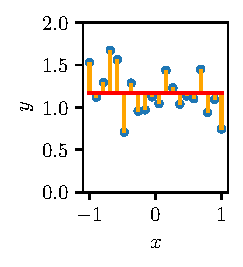
\includegraphics{const_opt.pdf}
\end{center}
And this optimal / best fitting predictor looks pretty good!

\subsection{Finding the best ``slope'' predictor}
Obviously, that was alot of work to just end up back at the mean.
But we confirmed that minimizing the sum-squared error loss does something sensible.
And we're going to be able to extend the sum-squared error loss idea to more complex cases.
The next step is to consider a predictor that only has one parameter, $w_2$, but depends on the data,
\begin{align}
  \yh_\text{slope}(x_i) &= w_2 x_i
\end{align}
Again, the loss can be written as a function of the parameter, $w_2$.
\begin{align}
  \L_\text{slope}(w_2) &= \sum_i \b{\yh_\text{slope}(x_i) - y_i}^2 =  \sum_i \b{w_2 x_i - y_i}^2.
\end{align} 
Our goal is to to find the prediction-function with the lowest loss.
To do that, we need to find the place where the derivative wrt $w_2$ is zero.
\begin{align}
  \dd[\L_\text{slope}(w_2)]{w_2} &= \dd{w_2} \sqb{\sum_{i=1}^N \b{w_2 x_i - y_i}^2}\\
  \intertext{we apply the chain rule, with $u_i = w_2 x_i - y_i$,}
  \L_\text{slope}(w_2) &= \sum_i u_i^2\\
  \dd[\L_\text{slope}(w_2)]{w_2} &= \sum_{i=1}^N \dd[u_i^2]{w_2} = \sum_{i=1}^N \dd[u_i^2]{u_i} \dd[u_i]{w_2} \\
  \intertext{the individual derivatives are,}
  \dd[u_i^2]{u_i} &= 2 u_i\\
  \dd[u_i]{w_2} &= \dd{w_2}\sqb{w_2 x_i - y_i} = x_i
  \intertext{Putting everything back together,}
  \dd[\L_\text{slope}(w_2)]{w_2} &= \sum_{i=1}^N \dd[u_i^2]{u_i} \dd[u_i]{w_2} = 2 \sum_{i=1}^N (w_2 x_i - y_i) x_i 
  \intertext{Now, we solve for the value of $w_2$ at which the gradient is zero,}
  0 &= \dd[\L_\text{slope}(w_2)]{w_2} = 2 \sum_{i=1}^N (w_2 x_i - y_i) x_i 
  \intertext{Expanding the bracket,}
  0 &= 2 \sum_{i=1}^N \b{- x_i y_i + w_2 x_i^2}\\
%\end{align}
%\begin{align}
%  \dd{w_2} \sqb{y_i^2} &= 0 & 
%  \dd{w_2} \sqb{-2 w_2 x_i y_i} &= - 2 x_i y_i &
%  \dd{w_2} \sqb{w_2^2} &= 2 w_2 x_i^2
%\end{align}
%so,
%\begin{align}
%  \dd{w_1} \sqb{\L_\text{slope}(w_1)} &= \sum_{i=1}^N \b{2 w_2 x_i^2 - 2 x_i y_i}
%\end{align}
%  \intertext{swap the derivative and sum,}
%  \dd{w_2} \sqb{\L_\text{const}(w_2)} &= \sum_{i=1}^N \dd{w_2} \b{w_2 x - y_i}^2\\
%  \intertext{we take,}
%  u_i &= w_2 x - y_i
%  \intertext{so the derivative of $\b{w_2 - y_i}^2$ is the derivative of $u_i^2$,}
%  \dd{w_2}\b{w_2 x - y_i}^2 &= \dd[u_i^2]{w_2} 
%  \intertext{and we can apply the chain rule,}
%  \dd[u_i^2]{u_i} = \dd[u_i]{w_2} \dd[u_i^2]{u_i}
%\end{align}
%where $u_i^2 = \b{w_2 - y_i}^2$. Now, we can compute the individual terms in the chain rule,
%\begin{align}
%  \dd[u_i]{w_2} &= \dd{w_2}[w_2 x_i - y_i] = x_i &
%  \dd[u_i^2]{u_i} &= 2 u_i = 2 \b{w_2 x - y_i}.
%\end{align}
%Putting all this back together, we get,
%\begin{align}
%  \dd{w_2}\b{w_2 - y_i}^2 &= \dd[u_i^2]{w_2} = \dd[u_i]{w_2} \dd[u_i^2]{u_i} = x_i \times 2 \b{w_2 x - y_i} = 2 x_i \b{w_2 x - y_i}.
%  \intertext{and the derivative of the loss becomes,}
%  \dd{w_2} \sqb{\L_\text{const}(w_2)} &= \sum_{i=1}^N 2 x_i \b{w_2 x_i - y_i}.
%\end{align}
%Now we solve for where the derivative is zero,
%\begin{align}
%  0 &= \sum_{i=1}^N \b{2 w_2 x_i^2 - 2 x_i y_i}
  \intertext{Divide both sides by $2$,}
  0 &= \sum_{i=1}^N \b{w_2 x_i^2 - y_i x_i}.
  \intertext{Now we sum over each term separately,}
  0 &= \sum_{i=1}^N w_2 x_i^2 - \sum_{i=1}^N y_i x_i.
  \intertext{Notice that $w_2$ doesn't depend on $i$, so it can be brought outside the sum,}
  0 &= w_2 \sum_{i=1}^N x_i^2 - \sum_{i=1}^N y_i x_i.
  \intertext{Now rearrange (add $\sum_{i=1}^N y_i x_i$ to both sides, and divide by $\sum_{i=1}^N x_i^2$,)}
  w_2 &= \frac{\sum_{i=1}^N y_i x_i}{\sum_{i=1}^N x_i^2}.
\end{align}
Does this make sense?  Yes! Remember that $w_2$ is the slope.  
The slope is bigger if for positive $x_i$, we have big positive $y_i$, and for negative $x_i$ we have big negative $y_i$.
And the numerator in this expression is big in exactly the same situation.

\subsection{Straight line fitting}
\label{sec:straight_line}
Above, we discussed the basic idea, but we only ever tried to fit a single parameter.
What happens when we fit a full straight line,
\begin{align}
  \yh(x_i) = w_1 + w_2 x_i
\end{align}
with an intercept, $w_1$ and slope, $w_2$ parameter?
Conceptually, it is the same idea we've seen previously: the loss is a function of $w_1$ and $w_2$,
\begin{align}
  \L(w_1, w_2) &= \sum_i \b{\yh(x_i) - y_i}^2 =  \sum_i \b{w_1 + w_2 x_i - y_i}^2
\end{align} 
We find the value of $w_1, w_2$ such that both derivatives are simultaneously zero,
\begin{align}
  0 &= \dd{w_1}\L(w_1, w_2) & 
  0 &= \dd{w_2}\L(w_1, w_2)
\end{align}
This is harder but still possible, so we're not going to give the proof here.

Instead, see the next section for a solution in an even more general setting.

%Instead, we're going to write down the solution for $w_2$, then give the implied value of $w_1$.
%Written in full, the optimal value of $w_2$,
%\begin{align}
%  w_2 &= \frac{\tfrac{1}{N} \sum_{i=1}^N x_i y_i - (\tfrac{1}{N} \sum_{i=1}^N x_i) (\tfrac{1}{N} \sum_{i=1}^N y_i)}{\tfrac{1}{N} \sum_i x_i^2 - (\tfrac{1}{N} \sum_i x_i)^2}\\
%  \intertext{As that's a bit painful, we can write it more succinctly as,}
%  w_2 &= \frac{\overline{x y} - \overline{x} \; \overline{y}}{\overline{x^2} - (\overline{x})^2}
%  \intertext{where,}
%  \overline{x y} &= \tfrac{1}{N} \sum_{i=1}^N x_i y_i\\
%  \overline{x} &= \tfrac{1}{N} \sum_{i=1}^N x_i\\
%  \overline{y} &= \tfrac{1}{N} \sum_{i=1}^N y_i\\
%  \overline{x^2} &= \tfrac{1}{N} \sum_{i=1}^N x_i^2\\
%  (\overline{x})^2 &= (\tfrac{1}{N} \sum_{i=1}^N x_i)^2
%\end{align}
%FYI: technically the ``overbar'' notation for sample averages and $\E{X}$ for ``true'' averages (e.g.\ when we define $X$ to be Gaussian with zero mean).  I (Laurence) will try to make this distinction, but it won't always happen!
%
%Now that we have $w_2$, we can solve for $w_1$.
%\begin{align}
%  0 &= \dd{w_1}\L_\text{slope}(w_1, w_2)\\
%  0 &= \dd{w_1}\sum_{i=1}^N \b{w_1 + w_2 x_i - y_i}^2\\
%  \intertext{Group all the terms that don't depend on $w_1$,}
%  0 &= \dd{w_1}\sum_{i=1}^N \b{w_1 + (w_2 x_i - y_i)}^2\\
%  \intertext{Expand the bracket (with all the terms that don't depend on $w_1$ in $\dotsm$),}
%  0 &= \dd{w_1}\sum_{i=1}^N \b{w_1^2 + 2 w_1 (w_2 x_i - y_i) + (w_2 x_i - y_i)^2}\\
%  \intertext{Take the derivative,}
%  0 &= \sum_{i=1}^N \sqb{2 w_1 + 2 (w_2 x_i - y_i)}\\
%  \intertext{Divide by two and put the sum inside the bracket,}
%  0 &= \sum_{i=1}^N w_1 - \sum_{i=1}^N (y_i - w_2 x_i)\\
%  \intertext{As $w_1$ does not vary with $i$,}
%  0 &= N w_1 - \sum_{i=1}^N (y_i - w_2 x_i).
%  \intertext{Adding $\sum_{i=1}^N (y_i - w_2 x_i)$ to both sides,}
%  N w_1 &= \sum_{i=1}^N (y_i - w_2 x_i).
%  \intertext{And dividing both sides by $N$,}
%  w_1 &= \tfrac{1}{N} \sum_{i=1}^N (y_i - w_2 x_i).
%\end{align}
%This makes sense: the intercept, $w_1$, is the average error between $y_i$ and $w_2 x_i$.  For instance, if $y_i$ is generally much bigger than $w_2 x_i$, then the intercept is positive.
%
%Overall, we have,
%\begin{subequations}
%  \label{eq:straight_line}
%  \begin{align}
%    w_2 &= \frac{\overline{x y} - \overline{x} \; \overline{y}}{\overline{x^2} - (\overline{x})^2}\\
%    w_1 &= \tfrac{1}{N} \sum_{i=1}^N (y_i - w_2 x_i).
%  \end{align}
%\end{subequations}

\section{Multivariable regression}
\label{sec:multi}

So far, we've always considered single-variable inputs, $x$, so that we can fit a curve on a 2D plot.
But in the real-world, we might want to predict an outcome from many features.
For instance, we might want to predict a product's sales from many different features (length, $x_1$, height, $x_2$, weight, $x_3$ etc.)
How can we do predictions with multiple input features?
To start with, we need to talk about how we're going to represent the data.
We say the data has $D$ features (e.g. for length, height, weight, we would have $D=3$ features) and $N$ datapoints. 
In that case, we could represent all the input features as an big $N \times D$ matrix, $\X$.
To give an example for $D = 3$.
\begin{align}
  \X &= \begin{pmatrix}
    X_{11} & X_{12} & X_{13}\\
    X_{21} & X_{22} & X_{23}\\
    \vdots & \vdots & \vdots\\
    X_{N1} & X_{N2} & X_{N3}\\
  \end{pmatrix}
  & 
  \y &= \begin{pmatrix}
    y_1\\
    y_2\\
    \vdots \\
    y_N\\
  \end{pmatrix} &
  \w &= \begin{pmatrix}
    w_1\\
    w_2\\
    w_3\\
  \end{pmatrix}
\end{align}
For both $\X$ and $\y$, each row corresponds to a datapoint. 
Thus, for each datapoint, we have an output $y_i$ and a row-vector of input features,

We could predict all outputs simultaneously, using,
\begin{align}
  \mathbf{\yh}(\X) = \X \w.
\end{align}
Alternatively, we could take the feature vector for a single datapoint (note this is a \textit{row} vector),
\begin{align}
  \x_i &= \begin{pmatrix} X_{i1} & X_{i2} & X_{i3} \end{pmatrix}
\end{align}
and make a prediction for a single datapoint,
\begin{align}
  \yh(\x_i) = \x_i \w = \sum_j X_{ij} w_j.
\end{align}
Note that this expression wouldn't work if $\x_i$ and $\w$ were both column vectors; it only works because $\x_i$ is a row-vector, and $\w$ is a column-vector.

The loss function is, as usual,
\begin{align}
  \mathcal{L}(\w) &= \sum_i \b{\yh(\x_i) - y_i}^2.
\end{align}
The optimal weights are,
\begin{align}
  \label{eq:wo}
  \wo &= \b{\X^T \X}^{-1} \X^T \y\\
  \intertext{I could give the derivation for this.  But its quite tedious, and isn't really super-relevant for later work in neural nets (as neural nets don't have analytic solutions like this).  Instead, I just want to make sure we think carefully about this expression and how the vectors/matrices in it work.  Specifically, lets look a bit closer at the sizes,}
  \underbrace{\wo}_{D \times 1} &= \big( \underbrace{\X^T}_{D\times N} \underbrace{\X}_{N \times D}\big)^{-1} \underbrace{\X^T}_{D \times N} \underbrace{\y}_{N \times 1}\\
  \intertext{Or, if we look at $\b{\X^T \X}^{-1}$ and $\X^T \y$ separately,}
  \underbrace{\wo}_{D \times 1} &= \underbrace{\b{\X^T \X}^{-1}}_{D \times D} \underbrace{\X^T \y}_{D \times 1}.
\end{align}
When doing this by hand, you'd usually compute $\b{\X^T \X}^{-1}$ and $\X^T \y$ first, as the number of dimensions, $D$, is usually going to be smaller than the number of datapoints (see Exercises for details).

The result will look something like,
\begin{center}
  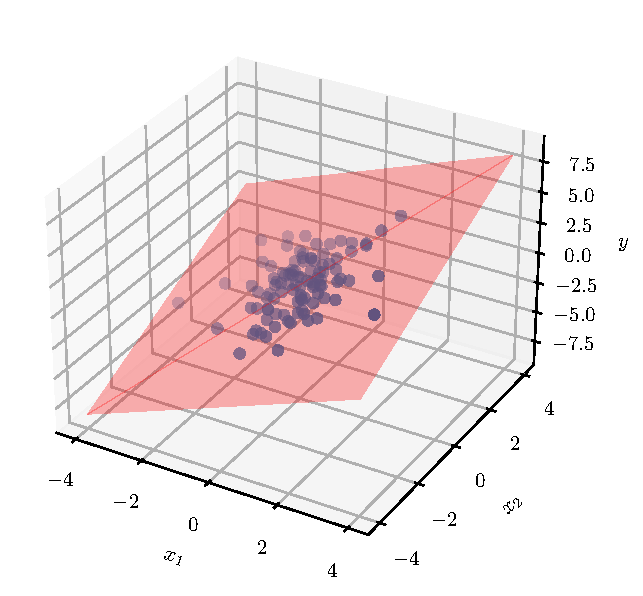
\includegraphics{multivariate.pdf}
\end{center}


\subsection{Regression with nonlinear features}

What if we want to fit a model of the form,
\begin{align}
  \label{eq:quad}
  \yh_\text{quad}(x) &= w_1 + w_2 x + w_3 x^2.
\end{align}
If we plot a bunch of these functions, with random $w_1$, $w_2$ and $w_3$, we get,
\begin{center}
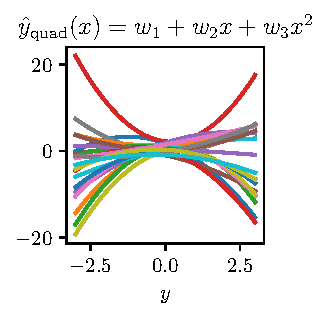
\includegraphics{quad_fam.pdf}
\end{center}

This is different from anything we've seen before because it is nonlinear: $\yh_\text{quad}(x)$ is a nonlinear function of $x$.
As such, it doesn't seem like anything we've done so far would help: we've only seen how to work with linear functions with a single or with multiple inputs.
However, it turns out that we can adapt the previous formula (for multivaraible regression) for this case.
The basic idea is to form multiple inputs for multivariable linear regression by applying a bunch of different functions (here, $f_1(\cdot)$, $f_2(\cdot)$ and $f_3(\cdot)$), to the actual input, $x_i$,
\begin{align}
  \label{eq:feat_vec}
  \x(x) &= \begin{pmatrix} f_1(x) & f_2(x) & f_3(x) \end{pmatrix}
\end{align}
So the big matrix $\X$ becomes,
\begin{align}
  \X &= \begin{pmatrix}
    f_1(x_1) & f_2(x_1) & f_3(x_1)\\
    f_1(x_2) & f_2(x_2) & f_3(x_2)\\
    \vdots & \vdots & \vdots\\
    f_1(x_N) & f_2(x_N) & f_3(x_N)\\
  \end{pmatrix}
\end{align}
Then, our prediction is a linear combination of the functions, $f_1(x)$, $f_2(x)$ and $f_3(x)$,
\begin{align}
  \label{eq:nonlin_yh}
  \yh(x) &= \x(x) \w = w_1 f_1(x) + w_2 f_2(x) + w_3 f_3(x).
\end{align}
To get back to our quadratic model (Eq.~\ref{eq:quad}), we choose,
\begin{align}
  f_1(x) &= 1\\
  f_2(x) &= x\\
  f_3(x) &= x^2
\end{align}
These choices for the functions give a feature vector (Eq.~\ref{eq:feat_vec}) of,
\begin{align}
  \x(x) &= \begin{pmatrix} 1 & x & x^2 \end{pmatrix}
\end{align}
That gives a big matrix of the form,
\begin{align}
  \X &= \begin{pmatrix}
    1 & x_1 & x_1^2\\
    1 & x_2 & x_2^2\\
    \vdots & \vdots & \vdots\\
    1 & x_N & x_N^2\\
  \end{pmatrix}
\end{align}
To get the optimal weights, we can plug this $\X$ and the usual outputs, $\y$ into Eq.~\eqref{eq:wo}.
The resulting fitted line looks something like,
\begin{center}
  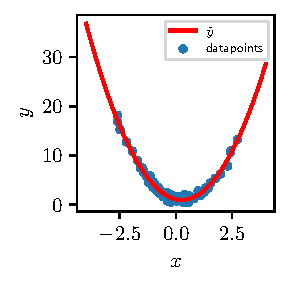
\includegraphics{quad.pdf}
\end{center}

\section{Gradient descent}

In the last part, we looked at analytic solutions.
However, analytic solutions are available in very few settings.
Instead, the approach taken in NNs is ``gradient descent'': computing the gradient of the loss wrt the parameters, then changing the parameters in the direction of minus the gradient, to reduce the loss.
Inuitively, we're following the gradient downhill, until we find the minimum.
\begin{center}
  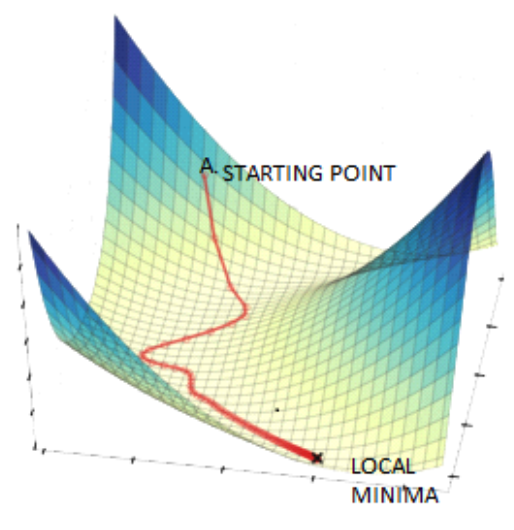
\includegraphics[width=0.4\textwidth]{grad_descent}
\end{center}

Mathematically, the updates to the weight are,
\begin{align}
  \Delta w_i &= - \eta \dd[\L]{w_i}
\end{align}
where $\eta$ is the learning rate, which is typically small (e.g.\ we might use $\eta=0.1$).  Note that the minus-sign is there, because the gradients point uphill, while we want to go downhill.

If you repeat this process, you should eventually end up at a place where the gradients are zero, at which point gradient descent will stop moving (remember that in the previous part, we were solving for the location where the gradients were zero).

\section{Gradient descent for linear regression}

So what do the actual gradient descent updates look like for linear regression?
Remember that in linear regression, we are fitting a straight line of the form,
\begin{align}
  \label{eq:grad:straight}
  \yh(x_i) = w_1 + w_2 x_i
\end{align}
with an intercept, $w_1$ and slope, $w_2$ parameter.
Conceptually, it is the same idea we've seen previously: the loss is a function of $w_1$ and $w_2$,
\begin{align}
  \L(w_1, w_2) &= \sum_i \b{\yh(x_i) - y_i}^2
\end{align} 
Now, we differentiate the loss wrt $w_1$,
\begin{align}
  \dd{w_1}\L(w_1, w_2) &= \sum_i \b{\yh(\x_i) - y_i}^2.
  \intertext{Now we use the chain rule, with $u_i=\yh(x_i) - y_i =w_1 + w_2 x_i - y_i$ (the final equality comes from substituting Eq.~\ref{eq:grad:straight}).  With this choice of $u_i$,}
  \L(\w) &= \sum_i u_i^2.
  \intertext{So,}
  \dd{w_1}\L(w_1, w_2) &= \sum_i \dd[u_i^2]{w_1} = \sum_i \dd[u_i^2]{u_i}\dd[u_i]{w_1}\\
  \intertext{The individual derivatives are,}
  \dd[u_i^2]{u} &= 2u_i = 2\b{\yh(x_i) - y_i}\\
  \dd[u_i]{w_1} &= \dd{w_1}\b{w_1 + w_2 x_i - y_i} = 1
  \intertext{Putting everything together,}
  \dd{w_1}\L(w_1, w_2) &= \sum_i \dd[u_i^2]{u_i}\dd[u_i]{w_2} = 2\sum_i \b{\yh(x_i) - y_i}
  \intertext{and finally our update is,}
  \Delta w_1 &= - \eta \dd{w_1}\L(w_1, w_2) \\
  &= 2 \eta \sum_i \b{y_i - \yh(x_i)}
\end{align}
These updates make sense: if the real data, $y_i$, is generally higher than our prediction, $\yh(x_i)$, then we should increase the bias, which increases all our predictions.

Now, we apply the same idea to $w_2$.
We use the same choice of $u_i$, so we can start at,
\begin{align}
  \dd{w_2}\L(w_1, w_2) &= \sum_i \dd[u_i^2]{w_2} = \sum_i \dd[u_i^2]{u_i}\dd[u_i]{w_2}\\
  \intertext{The individual derivatives are,}
  \dd[u_i^2]{u_i} &= 2u_i = 2\b{\yh(x_i) - y_i}\\
  \dd[u_i]{w_2} &= \dd{w_2}\b{w_1 + w_2 x_i - y_i} = x_i
  \intertext{Putting everything together,}
  \dd{w_1}\L(w_1, w_2) &= \sum_i \dd[u_i^2]{u_i}\dd[u_i]{w_2} = 2\sum_i x_i \b{\yh(x_i) - y_i}
  \intertext{and finally our update is,}
  \Delta w_2 &= - \eta \dd{w_1}\L(w_1, w_2) \\
  &= 2 \eta \sum_i x_i \b{y_i - \yh(x_i)}
\end{align}
To interpret these updates, consider a setting where again, the data, $y_i$, is bigger than our prediction, $\yh(x_i)$.
If $x_i$ is positive, then we can reduce the error by \textit{increasing} $w_2$ (as that will increase the size of $w_2 x_i$ in the predcition Eq.~\ref{eq:grad:straight}); and that's exactly what these updates do.
In contrast, if $x_i$ is negative, then we can reduce the error by \textit{decreasing} $w_2$, as that will make $w_2 x_i$ more positive.

\section{Gradient descent for multivariate linear regression}
Critically, gradient descent is much easier to generalise to more complex cases than analytic solutions, like those in the previous part.
As such, we can now derive the updates for multivariate linear regression (note that while there was an analytic solution in this case, we didn't derive it because its painful and not particularly instructive).
From last time, the prediction in multivariate linear regression was a weighted sum of features,
\begin{align}
  \yh(\x_i) = \x_i \w = \sum_\lambda X_{i\lambda} w_\lambda
\end{align}
We use the usual squared-error loss,
\begin{align}
  \L(\w) &= \sum_i \b{\yh(\x_i) - y_i}^2 = \sum_i \b{\sum_\lambda X_{i\lambda} w_\lambda - y_i}^2
\end{align}
Note that I have used $i$ to index datapoints, and $\lambda$ to index features.
Now, we differentiate wrt an individual weight,
\begin{align}
  \dd[\L(\w)]{w_\nu} &= \sum_i \dd{w_\nu} \b{\sum_\lambda X_{i\lambda} w_\lambda - y_i}^2.
  \intertext{As before, we apply the chain rule, with $u_i = \yh(x_i) - y_i =\sum_\lambda X_{i\lambda} w_\lambda - y_i$.  With this choice of $u_i$,}
  \L(\w) &= \sum_i u_i^2.
  \intertext{So,}
  \dd[\L(\w)]{w_\nu} &= \sum_i \dd[u_i^2]{w_\nu} = \sum_i \dd[u_i^2]{u_i} \dd[u_i]{w_\nu}\\
  \intertext{The individual derivatives are,}
  \dd[u_i^2]{u_i} &= 2u_i = 2\b{\yh(x_i) - y_i}\\
  \dd[u_i]{w_\nu} &= \dd{w_\nu}\b{\sum_\lambda X_{i\lambda} w_\lambda - y_i}
  \intertext{But this time, we need to think a bit more about the $\dd[u_i]{w_\nu}$. In particular, the gradient of $X_{i\lambda}$ and $y_i$ wrt $w_\nu$ is zero, as $X_{i\lambda}$ and $y_i$ are data, and data is fixed!}
  \dd[u_i]{w_\nu} &= \sum_\lambda X_{i\lambda} \dd[w_\lambda]{w_\nu}
  \intertext{The gradient of $w_\lambda$ wrt $w_\nu$ is 1 when $\lambda=\nu$, and zero otherwise.  That means its the Kronecker delta (see Part 1, mathematical prerequisites!)}
  \dd[u_i]{w_\nu} &= \sum_\lambda X_{i\lambda} \delta_{\lambda\nu}
  \intertext{As discussed in the prerequistes, the Kronecker delta picks out one component of the sum, where $\lambda=\nu$,}
  \dd[u_i]{w_\nu} &= X_{i\nu}.
  \intertext{Putting everything back together,}
  \dd[\L(\w)]{w_\nu} &= \sum_i \dd[u_i^2]{u_i} \dd[u_i]{w_\nu} = 2\sum_i \b{\yh(x_i) - y_i} X_{i \nu}.
  \intertext{So our gradient descent updates are,}
  \Delta w_\nu &= -\eta \dd[\L(\w)]{w_\nu} = 2 \eta \sum_i \b{y_i - \yh(x_i)} X_{i \nu}.
\end{align}
These updates again make sense.  If $X_{i\nu}$ is positive, and the error, $y_i - \yh(x_i)$, then increasing $w_{\nu}$ will reduce the error.

%\section{Regularisation}
%We saw (on the Python Notebook) that functions that are too complex can lead to overfitting.
%One approach to mitigating overfitting is to use ``regularisation''.
%So far, we have been minimizing the following loss problem,
%\begin{align}
%  \L(\w) &= \sum_{i=1}^N (y_i - \hat{y}(x_i))^2 = \sum_{i=1}^N (y_i - \w^T \x(x_i))^2.
%\end{align}
%That miminimizes the squared distance between real data, $y_i$, and predictions, $\hat{y}(x_i)$.
%However, it doesn't tell us anything about what happens outside the training datapoints, $(x_1,x_2,\dotsc,x_N)$.
%And the whole point is to do well outside of the training datapoints.
%One of the observations from the Notebook was that when our predictions go crazy (i.e.\ they get really big away from the training points) the weights also go crazy (i.e.\ they get really big).
%One approach to mitigating overfitting is therefore to add a term to the objective which penalises very large weights,
%\begin{align}
%  \L(\w) &= \sum_{i=1}^N (y_i - \w^T \x(x_i))^2 + \lambda \sum_{i=1}^D w_i^2.
%\end{align}
%The optimal weights are now very similar to, but slightly different from the original optimal weights (in Eq.~\ref{eq:wo})
%\begin{align}
%  \label{eq:wo_reg}
%  \wo &= \b{\X^T \X + \lambda \I}^{-1} \X^T \y
%\end{align}




\section{Exercises}
All these exercises are designed to be possible by hand (with a calculator).  We'd advise doing them that way, as that's how the exam will be set!

The following three exercises are based on this dataset.

\begin{center}
\begin{tabular}{c c}
  \toprule
  x & y \\
  \midrule
  -2 & -6.2\\
  -1 & -2.6\\
  0 &  0.5\\
  1 & 2.7\\
  2 & 5.7\\
  \bottomrule
\end{tabular}
\end{center}

\begin{exercise}
  Which of the following predictions has the lowest loss (specifically, the sum-squared distance),
  \begin{align}
    \hat{y}_1(x) &= x\\
    \hat{y}_2(x) &= 2 x\\
    \hat{y}_3(x) &= 3 x
  \end{align}
\end{exercise}

\begin{exercise}
  Fit a straight line of the form,
  \begin{align}
    \label{eq:q3_yh}
    \hat{y}(x) &= w_1 + w_2 x
  \end{align}
  using the formulae in Sec.~\ref{sec:multi}.
  Specifically, use two features:
  \begin{align}
    f_1(x) &= 1 & 
    f_2(x) &= x
  \end{align}
\end{exercise}

\begin{exercise}
  Fit a nonlinear prediction of the form,
  \begin{align}
    \label{eq:q4_yh}
    \hat{y}(x) &= w_1 x + w_2 x^2.
  \end{align}
  Again, use the formulae in Sec.~\ref{sec:multi}.  What $f_1$ and $f_2$ do you need to use?
\end{exercise}

\begin{exercise}
  The absolute value is defined as,
  \begin{align}
  |x| &= \begin{cases}
    x & \text{if } x>0\\
    -x & \text{otherwise}.
  \end{cases}
  \end{align}
  Sketch a plot of $y = |x|$, and compute,
  \begin{align}
    \dd[|x|]{x}  
  \end{align}
  Compute the gradient separately for $0 < x$ and $x < 0$. Don't worry about $x=0$, where the gradient is undefined.  And consider using the sign function,
  \begin{align}
    \operatorname{sign}(x) &= \begin{cases}
      1 &\textrm{if } 0 < x\\
      0 &\textrm{if } 0 = x\\
      -1 &\textrm{if } x < 0
    \end{cases}
  \end{align}
\end{exercise}

\begin{exercise}
  We have $N$ datapoints, $x_i$.
  We seek to find a location, $b$, which minimizes the sum of distances (not squared distances) between each datapoint, $x_i$ and $b$.
  Specifically, our loss function is,
  \begin{align}
    \L(b) &= \sum_{i=1}^N |x_i - b|,
  \end{align}
  Part 1: Compute the gradient of this following loss function, wrt $b$.  Write your answer in terms of the $\operatorname{sign}$ function (see answer to the prevous question for details).

  Part 2: Rewrite the gradient in words in terms of the number of datapoints above and below $b$.

  Part 3: Give an interpretation of the optimal value of $b$ (i.e.\ the value of $b$ for which the gradient is zero).  This is going to be easiest when there is an odd number of datapoints.
\end{exercise}

\section{Answers}

\begin{answer}
  Remember, the goal was to find which of the following prediction functions,
  \begin{align}
    \hat{y}_1(x) &= x\\
    \hat{y}_2(x) &= 2 x\\
    \hat{y}_3(x) &= 3 x
  \end{align}
  had the lowest loss.
  To do that, we need to evaluate the loss for $\hat{y}_1$, $\hat{y}_2$ and $\hat{y}_3$.  
  The predictions for $\hat{y}_1$ are,
  \begin{align}
    \hat{y}_1(x_1) &= x_1 = -2\\
    \hat{y}_1(x_2) &= x_2 = -1\\
    \hat{y}_1(x_3) &= x_3 = 0\\
    \hat{y}_1(x_4) &= x_4 = 1\\
    \hat{y}_1(x_5) &= x_5 = 2
  \end{align}
  Thus, the loss for $\hat{y}_1$ is  
  \begin{align}
    \L_1 &= \sum_{i=1}^5 (y_i - \hat{y}_1(x_i))^2\\
    \nonumber
    &= ((-6.2) - (-2))^2 + ((-2.6) - (-1))^2 + (0.5 - 0)^2 + (2.7 - 1)^2 + (5.7 - 2)^2\\
    &= (-4.2)^2 + (-1.6)^2 + (0.5)^2 + (1.7)^2 + (3.7)^2\\
    &= 37.03
  \end{align}
  The predictions for $\hat{y}_2$ are,
  \begin{align}
    \hat{y}_2(x_1) &= 2x_1 = 2\times(-2) = -4 \\
    \hat{y}_2(x_2) &= 2x_2 = 2\times(-1) = -2\\
    \hat{y}_2(x_3) &= 2x_3 = 2\times0 = 0\\
    \hat{y}_2(x_4) &= 2x_4 = 2\times1 = 2\\
    \hat{y}_2(x_5) &= 2x_5 = 2\times2 = 4
  \end{align}
  Thus, the loss for $\hat{y}_2$ is  
  \begin{align}
    \L_2 &= \sum_{i=1}^5 (y_i - \hat{y}_2(x_i))^2\\
    \nonumber
    &= ((-6.2) - (-4))^2 + ((-2.6) - (-2))^2 + (0.5 - 0)^2 + (2.7 - 2)^2 + (5.7 - 4)^2\\
    &= (-2.2)^2 + (-0.6)^2 + (0.5)^2 + (0.7)^2 + (1.7)^2\\
    &= 8.83
  \end{align}
  The predictions for $\hat{y}_3$ are,
  \begin{align}
    \hat{y}_3(x_1) &= 3x_1 = 3\times(-2) = -6 \\
    \hat{y}_3(x_2) &= 3x_2 = 3\times(-1) = -3\\
    \hat{y}_3(x_3) &= 3x_3 = 3\times0 = 0\\
    \hat{y}_3(x_4) &= 3x_4 = 3\times1 = 3\\
    \hat{y}_3(x_5) &= 3x_5 = 3\times2 = 6
  \end{align}
  Thus, the loss for $\hat{y}_3$ is  
  \begin{align}
    \L_3 &= \sum_{i=1}^5 (y_i - \hat{y}_3(x_i))^2\\
    \nonumber
    &= ((-6.2) - (-6))^2 + ((-2.6) - (-3))^2 + (0.5 - 0)^2 + (2.7 - 3)^2 + (5.7 - 6)^2\\
    &= (-0.2)^2 + (0.4)^2 + (0.5)^2 + (-0.3)^2 + (-0.3)^2\\
    &= 0.63
  \end{align}
  Overall, the three losses are:
  \begin{align}
    \L_1 &= 37.03\\
    \L_2 &= 8.83\\
    \L_3 &= 0.63
  \end{align}
  So the best (lowest loss) prediction is $\hat{y}_3$.  This makes sense if we e.g. sketch a plot of the data itself: the slope is about $3$.
\end{answer}


%\begin{answer}
%  We start by computing $w_2$ in Eq.~\eqref{eq:straight_line},
%  \begin{align}
%    w_2 &= \frac{\overline{x y} - \overline{x} \; \overline{y}}{\overline{x^2} - (\overline{x})^2}
%  \end{align}
%  That requires us to compute all the ``overbar'' quantities,
%  \begin{align}
%    \nonumber
%    \overline{x y} &= \tfrac{1}{N} \sum_{i=1}^N x_i y_i\\
%    \nonumber
%    &= \tfrac{1}{5} \b{(-2) {\times} (-6.2) + (-1) {\times} (-2.6) + 0 {\times} 0.5 + 1 {\times} 2.7 + 2{\times} 5.7}\\
%    \nonumber
%    &= \tfrac{1}{5} \b{12.4 + 2.6 + 0 + 2.7 + 10.4}\\
%    &= \tfrac{1}{5} 29.1 = 5.82.
%  \end{align}
%  \begin{align}
%    \nonumber
%    \overline{x} &= \tfrac{1}{N} \sum_{i=1}^N x_i\\
%    \nonumber
%    &= \tfrac{1}{5} \b{(-2) + (-1) + 0 + 1 + 2}\\
%    &= \tfrac{1}{5} \times 0 = 0
%  \end{align}
%  \begin{align}
%    \nonumber
%    \overline{y} &= \tfrac{1}{N} \sum_{i=1}^N y_i\\
%    \nonumber
%    &= \tfrac{1}{5} \b{(-6.2) + (-2.6) + 0.5 + 2.7 + 5.7}\\
%    &= \tfrac{1}{5} 0.1 = 0.02
%  \end{align}
%  \begin{align}
%    \nonumber
%    \overline{x^2} &= \tfrac{1}{N} \sum_{i=1}^N x_i^2\\
%    \nonumber
%    &= \tfrac{1}{5} \b{(-2)^2 + (-1)^2 + 0^2 + 1^2 + 2^2} \\
%    \nonumber
%    &= \tfrac{1}{5} \b{4 + 1 + 0 + 1 + 4}\\
%    &= \tfrac{1}{5} 10 = 2
%  \end{align}
%  Substituting these quantities into the formula for $w_2$, we get,
%  \begin{align}
%    w_2 &= \frac{5.82 - 0 \times 0.02}{2 - (0)^2} = \frac{5.82}{2} = 2.91
%  \end{align}
%  Now we can ask whether this is in the right ballpark.  The answer is yes.  Remember from the first question that we expected the slope to be about $3$ (e.g. if we sketch a plot of the data).
%
%  Now, we can compute $w_1$ in Eq.~\eqref{eq:straight_line},
%  \begin{align}
%    w_1 &= \tfrac{1}{N} \sum_{i=1}^N (y_i - w_2 x_i).
%  \end{align}
%  While we could compute this directly, with a little bit of manipulation, we can re-use our values for $\overline{y}$ and $\overline{x}$.
%  Specifically, we expand the bracket,
%  \begin{align}
%    w_1 &= \tfrac{1}{N} \sum_{i=1}^N y_i - w_2 \tfrac{1}{N} \sum_{i=1}^N x_i.
%    \intertext{Now, note that the first sum is $\overline{y}$ and the second sum is $\overline{x}$,}
%    w_1 &= \overline{y} - w_2 \overline{x}.\\
%    \intertext{Substituting the previously computed values of $\overline{y}$, $\overline{x}$, and $w_2$,}
%    w_1 &= 0.02 - 2.91 \times 0 = 0.02
%  \end{align}
%\end{answer}

\begin{answer}
  Remember that when we're doing regression with multiple features, our predictor is Eq.~\eqref{eq:nonlin_yh},
  \begin{align}
    \hat{y}(x) &= \x(x) \w = w_1 f_1(x) + w_2 f_2(x).
  \end{align}
  Substituting the $f_1(x)$ and $f_2(x)$ given in the question, we get back Eq.~\eqref{eq:q3_yh}, as we'd hope,
  \begin{align}
    \hat{y}(x) &= \x(x) \w = w_1 + w_2 x.
  \end{align}
  Now, we can compute the optimal weights using,
  \begin{align}
    \wo &= \b{\X^T \X}^{-1} \X^T \y.
  \end{align}
  To do that, we first need to construct the big feature matrix $\X$ and the big result vector, $\y$.
  The result vector is just a vector of the $y$'s
  \begin{align}
    \y &= \begin{pmatrix}
      y_1\\
      y_2\\
      y_3\\
      y_4\\
      y_5\\
    \end{pmatrix}
    = \begin{pmatrix}
      -6.2\\
      -2.6\\
       0.5\\
       2.7\\
       5.7
    \end{pmatrix}
  \end{align}
  We get the feature matrix, $\X$, by applying $f_1(\cdot)$ and $f_2(\cdot)$ to the $x$'s,
  \begin{align}
    \X &= \begin{pmatrix}
      f_1(x_1) & f_2(x_1)\\
      f_1(x_2) & f_2(x_2)\\
      f_1(x_3) & f_2(x_3)\\
      f_1(x_4) & f_2(x_4)\\
      f_1(x_5) & f_2(x_5)\\
    \end{pmatrix}
    = \begin{pmatrix}
      1 & x_1\\
      1 & x_2\\
      1 & x_3\\
      1 & x_4\\
      1 & x_5\\
    \end{pmatrix}
    = \begin{pmatrix}
      1 & -2\\
      1 & -1\\
      1 & 0\\
      1 & 1\\
      1 & 2\\
    \end{pmatrix}
  \end{align}
  Now, in principle all we have to do is to substitute this form for $\X$ and $\y$ into the form for the optimal weights,
  \begin{align}
    \wo &= \b{\X^T \X}^{-1} \X^T \y.
  \end{align}
  However, it turns out that we can simplify the computation a bit if we think carefully about the order of operations.
  And it turns out this thinking is helpful if we're doing the computation by hand (e.g.\ in an exam) or at a large scale on a computer.
  Specifically, remember that 
  \begin{align}
    \underbrace{\wo}_{D \times 1} &= \underbrace{\b{\X^T \X}^{-1}}_{D \times D} \underbrace{\X^T \y}_{D \times 1}.
  \end{align}
  and that the number of features ($D=2$ in our case) is typically smaller than the number of datapoints ($N=5$ in our case).
  Thus, it is easiest to first compute $\b{\X^T \X}^{-1}$ as that's just a $2\times 2$ matrix, and to compute $\X^T \y$ as that's just a length 2 vector.
  Thus, we start by computing the two-by-two matrix, $\X^T \X$,
  \begin{align}
    \X^T \X &= 
    \begin{pmatrix}
      1 & 1 & 1 & 1 & 1\\
      -2 & -1 & 0 & 1 & 2
    \end{pmatrix}
    \begin{pmatrix}
      1 & -2\\
      1 & -1\\
      1 & 0\\
      1 & 1\\
      1 & 2\\
    \end{pmatrix}
    = \begin{pmatrix}
      5 & 0 \\ 0 & 10
    \end{pmatrix}
  \end{align}
  For instance, the top-left element is given by,
  \begin{align}
    5 &= 1 {\times} 1 + 1 {\times} 1 + 1 {\times} 1 + 1 {\times} 1 + 1 {\times} 1 = 1 + 1 + 1 + 1 + 1
    \intertext{For instance, and top-right element is given by,}
    0 &= 1 {\times} (-2) + 1 {\times} (-1) + 1 {\times} 0 + 1 {\times} 1 + 1 {\times} 2 = (-2) + (-1) + 0 + 1 + 2
  \end{align}
  We can then compute $\b{\X^T \X}^{-1}$ by using the usual formula for the $2 \times 2$ matrix inverse,
  \begin{align}
    \begin{pmatrix}
      a & b \\ c & d
    \end{pmatrix}^{-1} &= \frac{1}{ad - bc} \begin{pmatrix} d & -b \\ -c & a \end{pmatrix}
    \intertext{Thus,}
    \b{\X \X^T}^{-1} &=  \begin{pmatrix}
      5 & 0 \\ 0 & 10
    \end{pmatrix}^{-1} \\
    &= \frac{1}{5\times 10 - 0 \times 0} \begin{pmatrix} 10 & 0 \\ 0 & 5 \end{pmatrix} \\
    &= \frac{1}{50}\begin{pmatrix} 10 & 0 \\ 0 & 5 \end{pmatrix} \\
    &= \begin{pmatrix} \tfrac{1}{5} & 0 \\ 0 & \tfrac{1}{10} \end{pmatrix}
  \end{align}
  Next, we compute $\X^T \y$, which is a matrix-vector product,
  \begin{align}
    \X^T \y &= 
    \begin{pmatrix}
      1 & 1 & 1 & 1 & 1\\
      -2 & -1 & 0 & 1 & 2
    \end{pmatrix}
    \begin{pmatrix}
      -6.2\\
      -2.6\\
       0.5\\
       2.7\\
       5.7
    \end{pmatrix}\\
    &=
    \begin{pmatrix}
      {1 {\times} (-6.2) + 1 {\times} (-2.6) + 1 {\times} 0.5 + 1 {\times} 2.7 + 1{\times} 5.7}\\
      {(-2) {\times} (-6.2) + (-1) {\times} (-2.6) + 0 {\times} 0.5 + 1 {\times} 2.7 + 2{\times} 5.7}
    \end{pmatrix}\\
    &=
    \begin{pmatrix}
      {(-6.2) + (-2.6) + 0.5 + 2.7 + 5.7}\\
      {12.4 + 2.6 + 0 + 2.7 + 11.4}
    \end{pmatrix}\\
    &= 
    \begin{pmatrix}
      0.1\\
      29.1
    \end{pmatrix}
  \end{align}
  Now, we can substitute our values for $\b{\X^T \X}^{-1}$ and $\X^T \y$ into the form for the optimal weights,
  \begin{align}
    \wo &= \b{\X^T \X}^{-1} \X^T \y\\
    \begin{pmatrix}
      w_1\\
      w_2\\
    \end{pmatrix} &= 
    \begin{pmatrix} \tfrac{1}{5} & 0 \\ 0 & \tfrac{1}{10} \end{pmatrix}
    \begin{pmatrix}
      0.1\\
      29.1
    \end{pmatrix}
    = 
    \begin{pmatrix}
      0.02\\
      2.91
    \end{pmatrix}
  \end{align}
  So $w_1 = 0.02$ and $w_2 = 2.91$, which is exactly the same answer using the alternative strategy in the previous question!
\end{answer}

\begin{answer}
  Remember that when we're doing regression with multiple features, our predictor is (Eq.~\ref{eq:nonlin_yh}),
  \begin{align}
    \hat{y}(x) &= \x(x) \w = w_1 f_1(x) + w_2 f_2(x).
  \end{align}
  Looking back at Eq.~\eqref{eq:q4_yh},
  \begin{align}
    \hat{y}(x) &= w_1 x + w_2 x^2,
  \end{align}
  we need to choose,
  \begin{align}
    f_1(x) & = x & f_2(x) = x^2.
  \end{align}
  Now, we can compute the optimal weights using,
  \begin{align}
    \wo &= \b{\X^T \X}^{-1} \X^T \y.
  \end{align}
  To do that, we first need to construct the big feature matrix $\X$ and the big result vector, $\y$.
  The result vector is just a vector of the $y$'s
  \begin{align}
    \y &= \begin{pmatrix}
      y_1\\
      y_2\\
      y_3\\
      y_4\\
      y_5\\
    \end{pmatrix}
    = \begin{pmatrix}
      -6.2\\
      -2.6\\
       0.5\\
       2.7\\
       5.7
    \end{pmatrix}
  \end{align}
  We get the feature matrix, $\X$, by applying $f_1(\cdot)$ and $f_2(\cdot)$ to the $x_i$'s,
  \begin{align}
    \X &= \begin{pmatrix}
      f_1(x_1) & f_2(x_1)\\
      f_1(x_2) & f_2(x_2)\\
      f_1(x_3) & f_2(x_3)\\
      f_1(x_4) & f_2(x_4)\\
      f_1(x_5) & f_2(x_5)\\
    \end{pmatrix}
    = \begin{pmatrix}
      x_1 & x_1^2\\
      x_2 & x_2^2\\
      x_3 & x_3^2\\
      x_4 & x_4^2\\
      x_5 & x_5^2\\
    \end{pmatrix}
    = \begin{pmatrix}
      -2 & (-2)^2\\
      -1 & (-1)^2\\
      0 & 0^2\\
      1 & 1^2\\
      2 & 2^2\\
    \end{pmatrix}
    = \begin{pmatrix}
      -2 & 4\\
      -1 & 1\\
      0 & 0\\
      1 & 1\\
      2 & 4\\
    \end{pmatrix}
  \end{align}
  We start by computing the two-by-two matrix, $\X^T \X$,
  \begin{align}
    \X^T \X &= 
    \begin{pmatrix}
      -2 & -1 & 0 & 1 & 2\\
      4 & 1 & 0 & 1 & 4
    \end{pmatrix}
    \begin{pmatrix}
      -2 & 4\\
      -1 & 1\\
      0 & 0\\
      1 & 1\\
      2 & 4\\
    \end{pmatrix}
    = \begin{pmatrix}
      10 & 0 \\ 0 & 34
    \end{pmatrix}
  \end{align}
  We can then compute $\b{\X^T \X}^{-1}$ by using the usual formula for the $2 \times 2$ matrix inverse,
  \begin{align}
    \begin{pmatrix}
      a & b \\ c & d
    \end{pmatrix}^{-1} &= \frac{1}{ad - bc} \begin{pmatrix} d & -b \\ -c & a \end{pmatrix}
    \intertext{Thus,}
    \b{\X \X^T}^{-1} &=  \begin{pmatrix}
      10 & 0 \\ 0 & 34
    \end{pmatrix}^{-1} \\
    &= \frac{1}{10\times 34 - 0 \times 0} \begin{pmatrix} 34 & 0 \\ 0 & 10 \end{pmatrix} \\
    &= \frac{1}{340}\begin{pmatrix} 34 & 0 \\ 0 & 10 \end{pmatrix} \\
    &= \begin{pmatrix} \tfrac{1}{10} & 0 \\ 0 & \tfrac{1}{34} \end{pmatrix}
  \end{align}
  Next, we compute $\X^T \y$, which is a matrix-vector product,
  \begin{align}
    \X^T \y &= 
    \begin{pmatrix}
      -2 & -1 & 0 & 1 & 2\\
      4 & 1 & 0 & 1 & 4
    \end{pmatrix}
    \begin{pmatrix}
      -6.2\\
      -2.6\\
       0.5\\
       2.7\\
       5.7
    \end{pmatrix}\\
    &=
    \begin{pmatrix}
      {(-2) {\times} (-6.2) + (-1) {\times} (-2.6) + 0 {\times} 0.5 + 1 {\times} 2.7 + 2{\times} 5.7}\\
      {4 {\times} (-6.2) + 1 {\times} (-2.6) + 0 {\times} 0.5 + 1 {\times} 2.7 + 4{\times} 5.7}
    \end{pmatrix}\\
    &= 
    \begin{pmatrix}
      29.1\\
      -1.9
    \end{pmatrix}
  \end{align}
  Now, we can substitute our values for $\b{\X^T \X}^{-1}$ and $\X^T \y$ into the form for the optimal weights,
  \begin{align}
    \wo &= \b{\X^T \X}^{-1} \X^T \y\\
    \begin{pmatrix}
      w_1\\
      w_2\\
    \end{pmatrix} &= 
    \begin{pmatrix} \tfrac{1}{10} & 0 \\ 0 & \tfrac{1}{34} \end{pmatrix}
    \begin{pmatrix}
      29.1\\
      -1.9
    \end{pmatrix}
    = 
    \begin{pmatrix}
      2.91\\
      -0.0559
    \end{pmatrix}
  \end{align}
  So $w_1 = 2.91$.  Remember that this is now the linear weight (i.e.\ the term that multiplies $x$). Surprisingly, it has the same value as we saw previously (this doesn't happen in general, and only occurs in this case because the off-diagonals of $\X^T \X$ are zero). Additionally, the quadratic weight, $w_2 = 0.0559$, is small.  That makes sense because the underlying data looks more like a straight line than a quadratic.
\end{answer}


\begin{answer}
  The sketch plot looks like:

  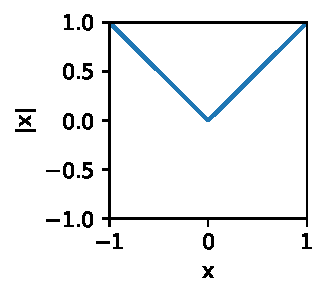
\includegraphics{abs.pdf}

  We can differentiate each ``case'' separately.
  \begin{align}
    \dd[| x |]{x} &= \begin{cases}
      \dd[x]{x} & \text{if } 0 < x\\
    \dd[-x]{x} & \text{if } x < 0
  \end{cases}\\
  &= \begin{cases}
     1 & \text{if } 0 < x\\
    -1 & \text{if } x < 0.
  \end{cases} \\
  &= \operatorname{sign}(x)
  \end{align}
  (If we play a little fast-and-loose with the zero.)

  FYI, there is no well-defined gradient at the ``kink'' (i.e.\ $x=0$), but that isn't really relevant in practice, so we aren't going to worry about it here.
\end{answer}

\begin{answer}
  Part 1 (gradient of $\L(b)$ in terms of $\operatorname{sign}$),
  \begin{align}
    \dd[\L(b)]{b} &= \sum_{i=1}^N \dd[|x_i - b|]{b} \\
    \intertext{use the chain rule with $u_i = x_i-b$,}
    \dd[\L(b)]{b} &= \sum_{i=1}^N \dd[|u_i|]{u_i} \dd[u_i]{b}\\
    \dd[\L(b)]{b} &= \sum_{i=1}^N \operatorname{sign}(x_i - b) (-1)\\
    \dd[\L(b)]{b} &= - \sum_{i=1}^N \operatorname{sign}(x_i - b).
  \end{align}
  Part 2 (interpretation in terms of the number of datapoints above and below a threshold):  
  \begin{align}
    \operatorname{sign}(x_i - b) &= 
    \begin{cases}
      1 & \text{if } b < x_i\\
      -1 & \text{if } x_i < b
    \end{cases}
  \end{align}
  Thus, the gradient of the loss in effect counts the number of datapoints above and below $b$,
  \begin{align}
    \dd[\L(b)]{b} &= (\text{Number of datapoints below } b) - (\text{Number of datapoints above } b).
  \end{align}
  Part 3: the optimal value of $b$ is at,
  \begin{align}
     0 &=\dd[\L(b)]{b} = (\text{Number of datapoints below } b) - (\text{Number of datapoints above } b).
  \end{align}
  i.e.\ this is a value of $b$ for which,
  \begin{align}
     (\text{Number of datapoints below } b) = (\text{Number of datapoints above } b)
  \end{align}
  And this value for $b$ is the median.

  FYI: There are some subtleties here about how exactly how we define the median.
  If there an odd number of datapoints, then the median really is the ``middle'' datapoint.
  If there an even number of datapoints, then there isn't a single ``middle'' datapoint: there's two.  Most computer implementations of the median would return halfway between the two middle datapoints.  But we have $0 =\dd[\L(b)]{b}$ for any $b$ between those two datapoints.  
\end{answer}

\end{document}

